\section{Results} \label{sc:results}
Ȉric: setting this section offline (due to Overleaf limitation). Available in GitHub

\subsection{Synthetic images}

\subsubsection{KSVD}

\begin{figure}[H]
  \centering
  \begin{tabular}{c c c c c}
      \begin{varwidth}{0.5\linewidth}
        \subfigure{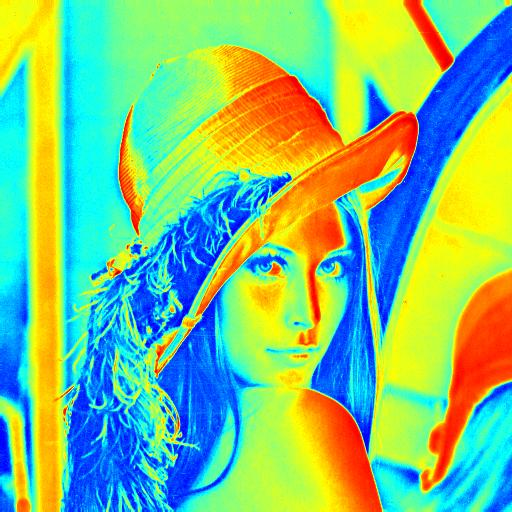
\includegraphics[width=16mm]{Experiments_synthetic_images/color_lena.jpg}}\\
        \subfigure{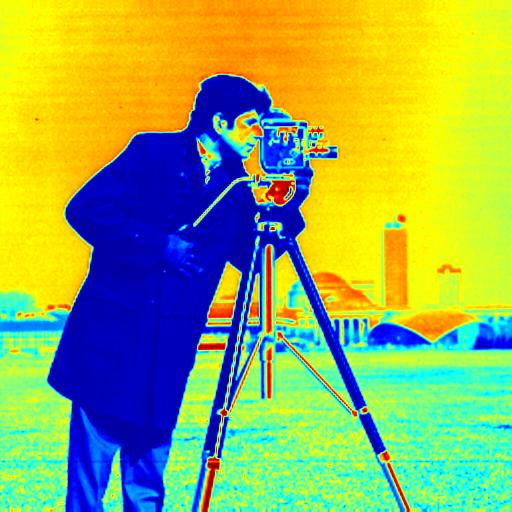
\includegraphics[width=16mm]{Experiments_synthetic_images/color_cameraman.jpg}}\\
        \subfigure{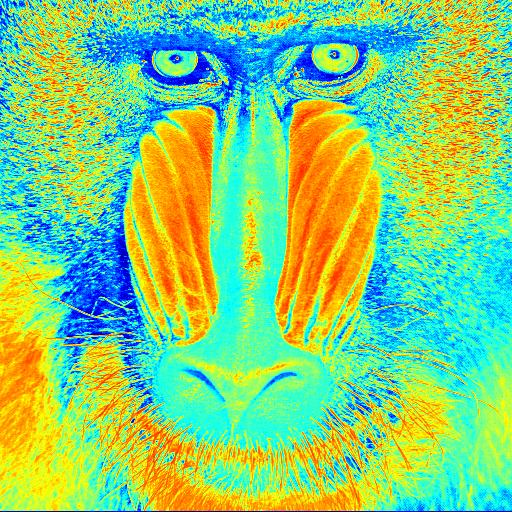
\includegraphics[width=16mm]{Experiments_synthetic_images/color_baboon.jpg}}
      \end{varwidth}
      \begin{varwidth}{0.5\linewidth}
        \subfigure{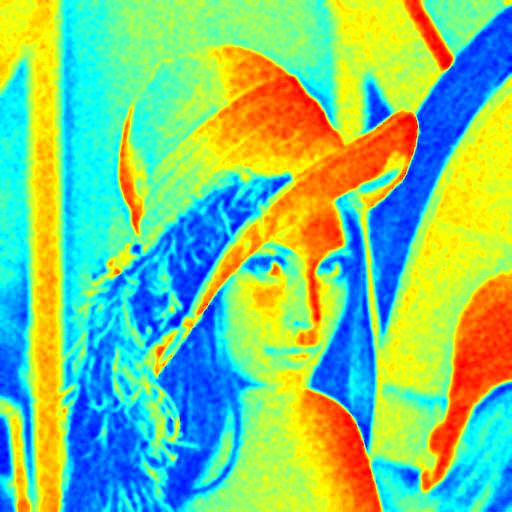
\includegraphics[width=16mm]{Results_KSVD/color_lena_nor.jpg}}\\
        \subfigure{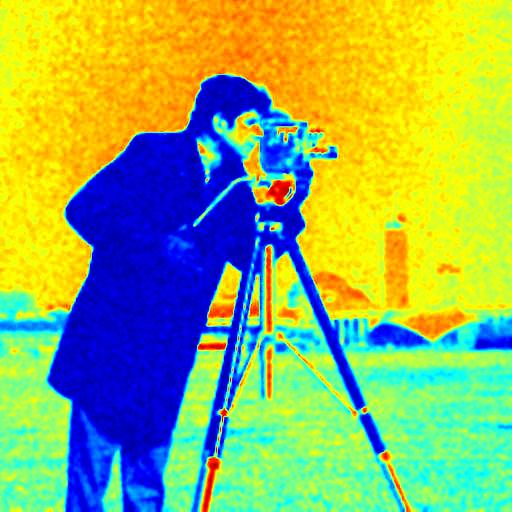
\includegraphics[width=16mm]{Results_KSVD/color_cameraman_nor.jpg}}\\
        \subfigure{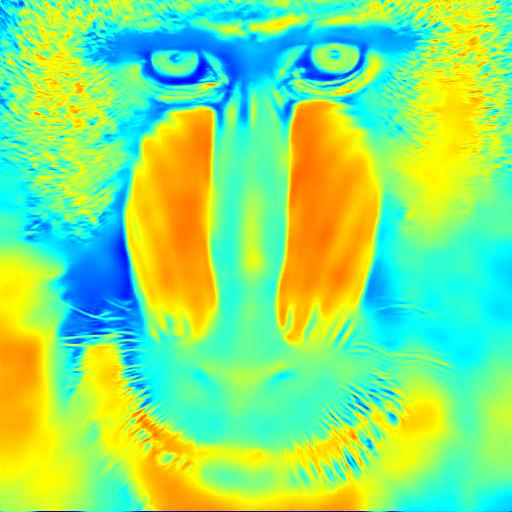
\includegraphics[width=16mm]{Results_KSVD/color_baboon_nor.jpg}}
      \end{varwidth}
      \begin{varwidth}{0.5\linewidth}
        \subfigure{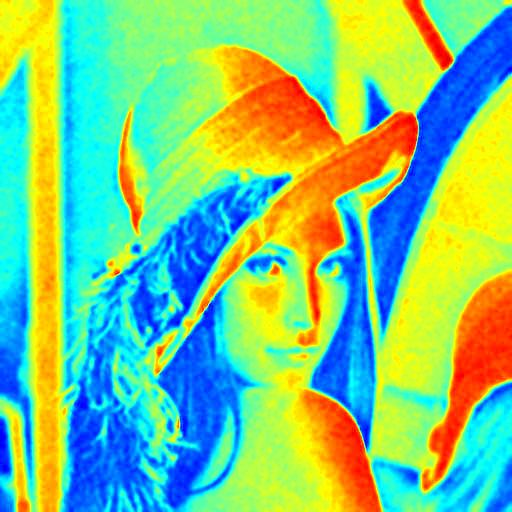
\includegraphics[width=16mm]{Results_KSVD/color_lena_ric.jpg}}\\
        \subfigure{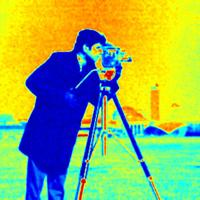
\includegraphics[width=16mm]{Results_KSVD/color_cameraman_ric.jpg}}\\
        \subfigure{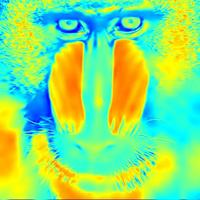
\includegraphics[width=16mm]{Results_KSVD/color_baboon_ric.jpg}}
      \end{varwidth}
      \begin{varwidth}{0.5\linewidth}
        \subfigure{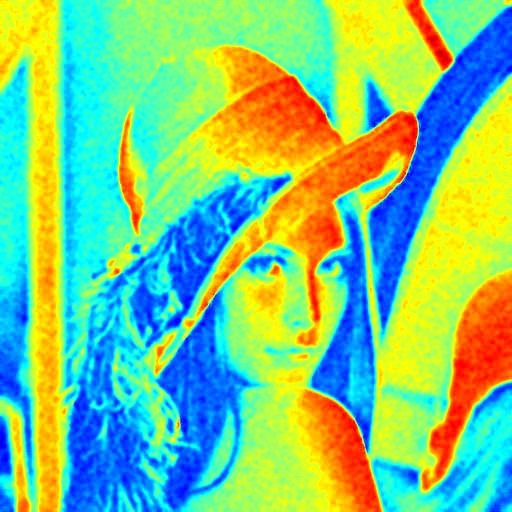
\includegraphics[width=16mm]{Results_KSVD/color_lena_uni.jpg}}\\
        \subfigure{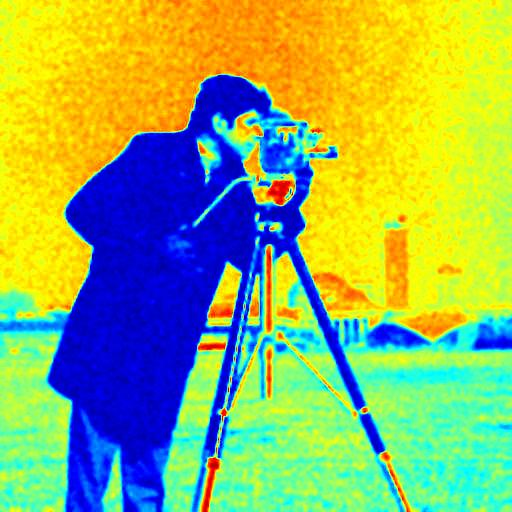
\includegraphics[width=16mm]{Results_KSVD/color_cameraman_uni.jpg}}\\
        \subfigure{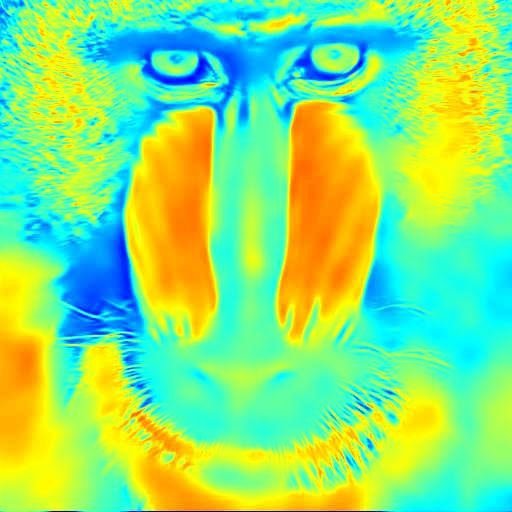
\includegraphics[width=16mm]{Results_KSVD/color_baboon_uni.jpg}}
      \end{varwidth}
      \begin{varwidth}{0.5\linewidth}
        \subfigure{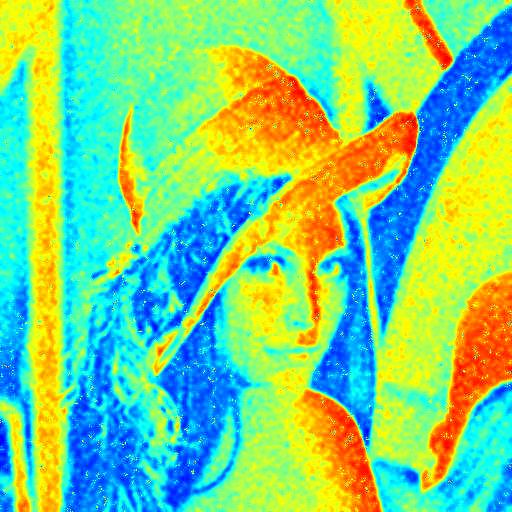
\includegraphics[width=16mm]{Results_KSVD/color_lena_sp.jpg}}\\
        \subfigure{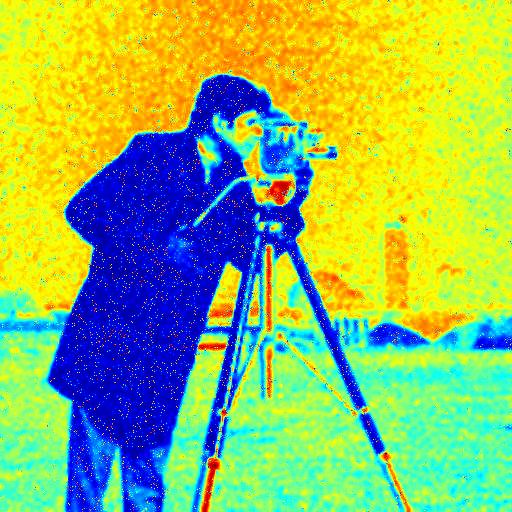
\includegraphics[width=16mm]{Results_KSVD/color_cameraman_sp.jpg}}\\
        \subfigure{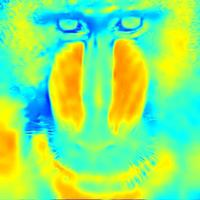
\includegraphics[width=16mm]{Results_KSVD/color_baboon_sp.jpg}}
      \end{varwidth}
  	\end{tabular}
  \caption{} 
  \label{fig:results_ksvd_c}
\end{figure}

\subsubsection{Mean filter}

\begin{figure}[H]
  \centering
  \begin{tabular}{c c c c c}
      \begin{varwidth}{0.5\linewidth}
        \subfigure{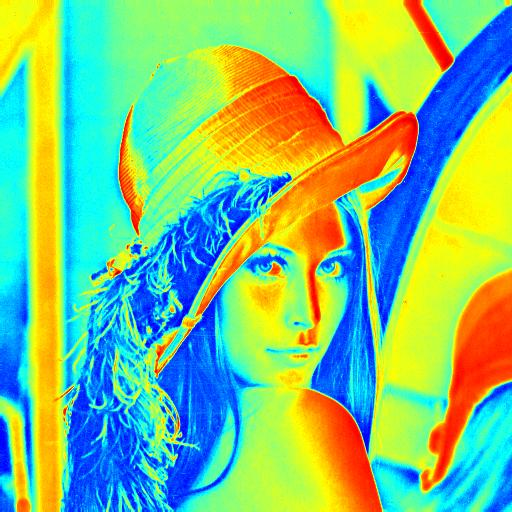
\includegraphics[width=16mm]{Experiments_synthetic_images/color_lena.jpg}}\\
        \subfigure{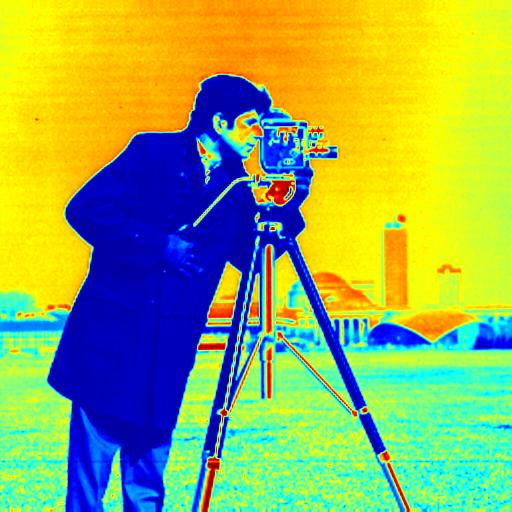
\includegraphics[width=16mm]{Experiments_synthetic_images/color_cameraman.jpg}}\\
        \subfigure{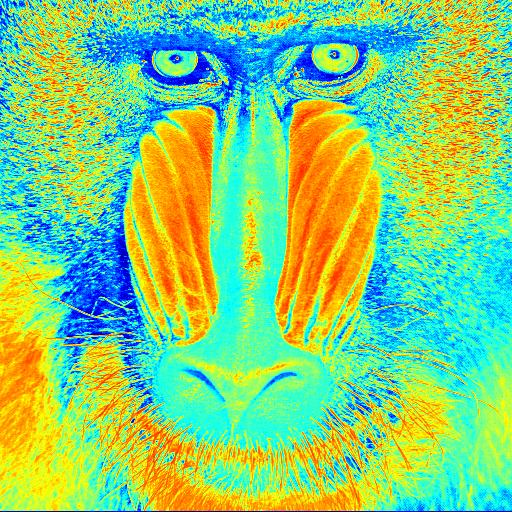
\includegraphics[width=16mm]{Experiments_synthetic_images/color_baboon.jpg}}
      \end{varwidth}
      \begin{varwidth}{0.5\linewidth}
        \subfigure{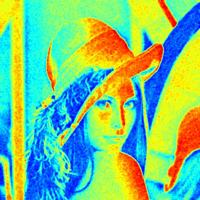
\includegraphics[width=16mm]{Results_mean/color_lena_nor_f.jpg}}\\
        \subfigure{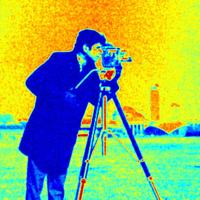
\includegraphics[width=16mm]{Results_mean/color_cameraman_nor_f.jpg}}\\
        \subfigure{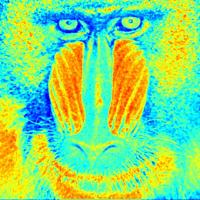
\includegraphics[width=16mm]{Results_mean/color_baboon_nor_f.jpg}}
      \end{varwidth}
      \begin{varwidth}{0.5\linewidth}
        \subfigure{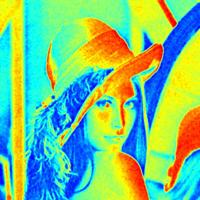
\includegraphics[width=16mm]{Results_mean/color_lena_ric_f.jpg}}\\
        \subfigure{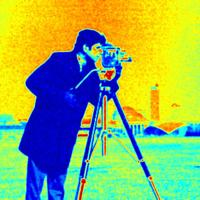
\includegraphics[width=16mm]{Results_mean/color_cameraman_ric_f.jpg}}\\
        \subfigure{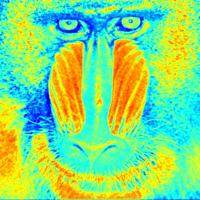
\includegraphics[width=16mm]{Results_mean/color_baboon_ric_f.jpg}}
      \end{varwidth}
      \begin{varwidth}{0.5\linewidth}
        \subfigure{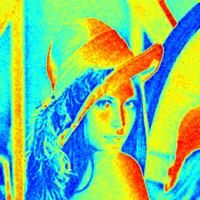
\includegraphics[width=16mm]{Results_mean/color_lena_uni_f.jpg}}\\
        \subfigure{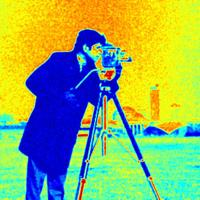
\includegraphics[width=16mm]{Results_mean/color_cameraman_uni_f.jpg}}\\
        \subfigure{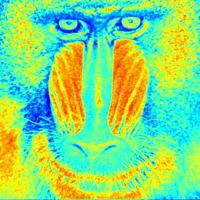
\includegraphics[width=16mm]{Results_mean/color_baboon_uni_f.jpg}}
      \end{varwidth}
      \begin{varwidth}{0.5\linewidth}
        \subfigure{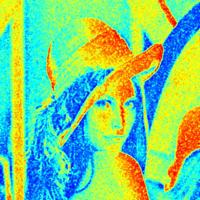
\includegraphics[width=16mm]{Results_mean/color_lena_sp_f.jpg}}\\
        \subfigure{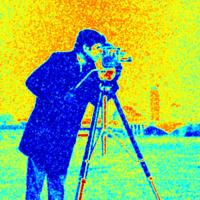
\includegraphics[width=16mm]{Results_mean/color_cameraman_sp_f.jpg}}\\
        \subfigure{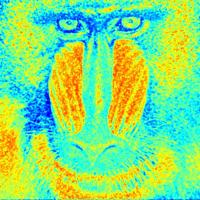
\includegraphics[width=16mm]{Results_mean/color_baboon_sp_f.jpg}}
      \end{varwidth}
  	\end{tabular}
  \caption{} 
  \label{fig:results_mean_c}
\end{figure}

compare with KSVD results

\subsubsection{Median filter}

\begin{figure}[H]
  \centering
  \begin{tabular}{c c c c c}
      \begin{varwidth}{0.5\linewidth}
        \subfigure{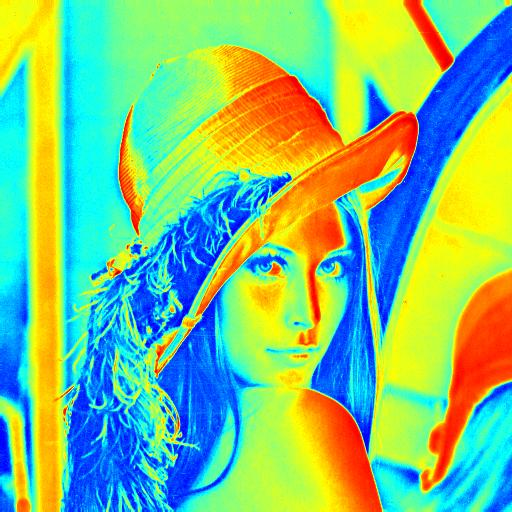
\includegraphics[width=16mm]{Experiments_synthetic_images/color_lena.jpg}}\\
        \subfigure{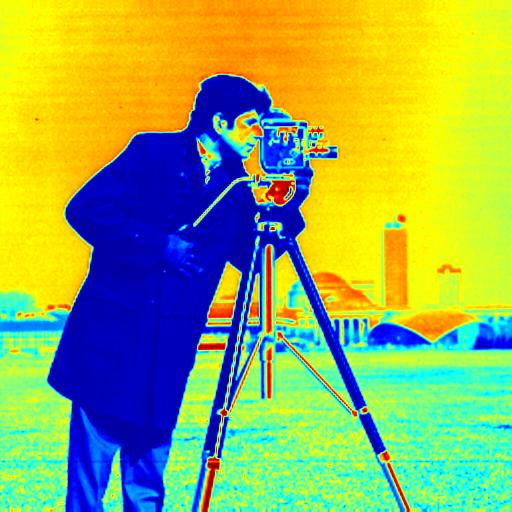
\includegraphics[width=16mm]{Experiments_synthetic_images/color_cameraman.jpg}}\\
        \subfigure{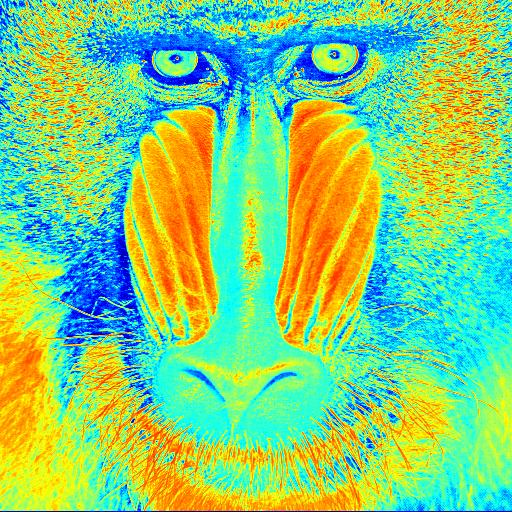
\includegraphics[width=16mm]{Experiments_synthetic_images/color_baboon.jpg}}
      \end{varwidth}
      \begin{varwidth}{0.5\linewidth}
        \subfigure{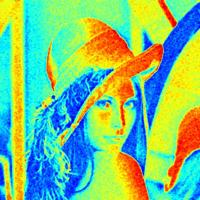
\includegraphics[width=16mm]{Results_median/color_lena_nor_f.jpg}}\\
        \subfigure{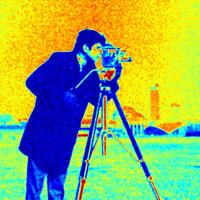
\includegraphics[width=16mm]{Results_median/color_cameraman_nor_f.jpg}}\\
        \subfigure{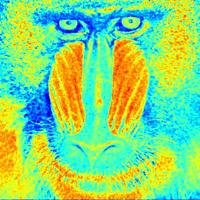
\includegraphics[width=16mm]{Results_median/color_baboon_nor_f.jpg}}
      \end{varwidth}
      \begin{varwidth}{0.5\linewidth}
        \subfigure{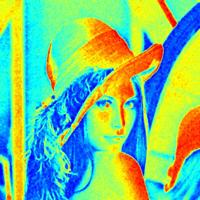
\includegraphics[width=16mm]{Results_median/color_lena_ric_f.jpg}}\\
        \subfigure{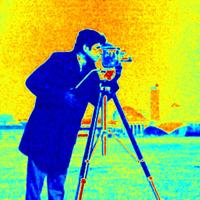
\includegraphics[width=16mm]{Results_median/color_cameraman_ric_f.jpg}}\\
        \subfigure{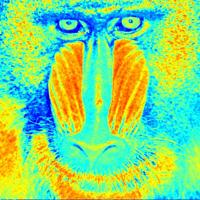
\includegraphics[width=16mm]{Results_median/color_baboon_ric_f.jpg}}
      \end{varwidth}
      \begin{varwidth}{0.5\linewidth}
        \subfigure{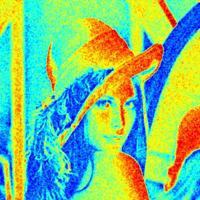
\includegraphics[width=16mm]{Results_median/color_lena_uni_f.jpg}}\\
        \subfigure{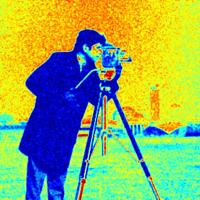
\includegraphics[width=16mm]{Results_median/color_cameraman_uni_f.jpg}}\\
        \subfigure{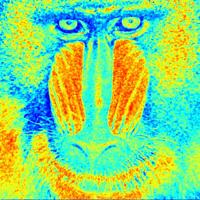
\includegraphics[width=16mm]{Results_median/color_baboon_uni_f.jpg}}
      \end{varwidth}
      \begin{varwidth}{0.5\linewidth}
        \subfigure{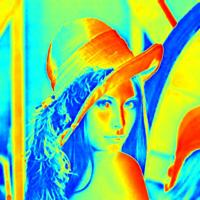
\includegraphics[width=16mm]{Results_median/color_lena_sp_f.jpg}}\\
        \subfigure{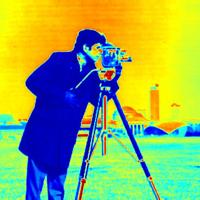
\includegraphics[width=16mm]{Results_median/color_cameraman_sp_f.jpg}}\\
        \subfigure{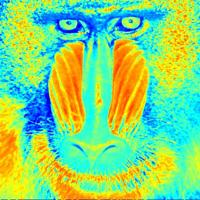
\includegraphics[width=16mm]{Results_median/color_baboon_sp_f.jpg}}
      \end{varwidth}
  	\end{tabular}
  \caption{} 
  \label{fig:results_median_c}
\end{figure}

compare with KSVD results

\subsubsection{Lee filter}

\begin{figure}[H]
  \centering
  \begin{tabular}{c c c c c}
      \begin{varwidth}{0.5\linewidth}
        \subfigure{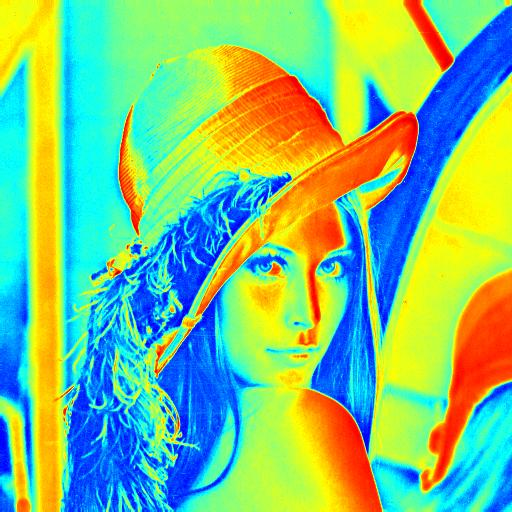
\includegraphics[width=16mm]{Experiments_synthetic_images/color_lena.jpg}}\\
        \subfigure{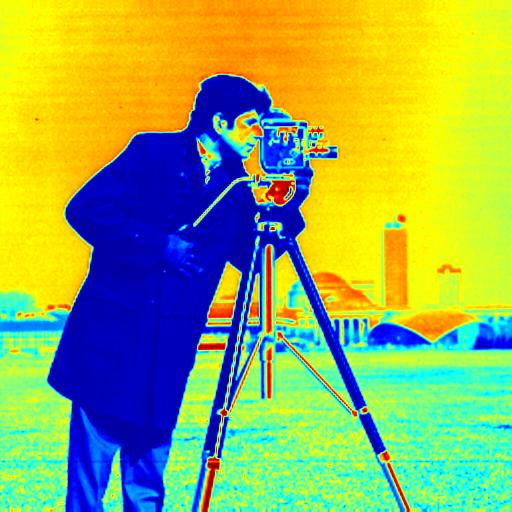
\includegraphics[width=16mm]{Experiments_synthetic_images/color_cameraman.jpg}}\\
        \subfigure{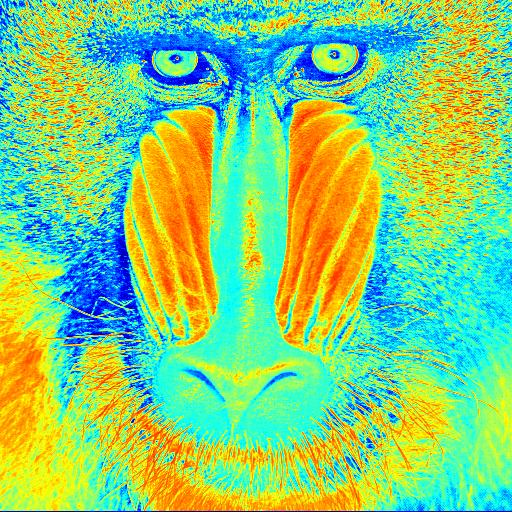
\includegraphics[width=16mm]{Experiments_synthetic_images/color_baboon.jpg}}
      \end{varwidth}
      \begin{varwidth}{0.5\linewidth}
        \subfigure{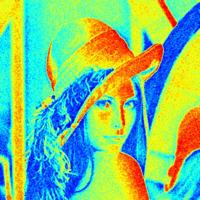
\includegraphics[width=16mm]{Results_Lee/color_lena_nor-denoised.jpg}}\\
        \subfigure{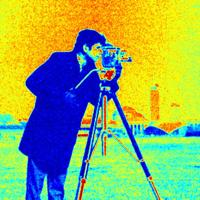
\includegraphics[width=16mm]{Results_Lee/color_cameraman_nor-denoised.jpg}}\\
        \subfigure{\includegraphics[width=16mm]{Results_Lee/color_baboon_nor-denoised.jpg}}
      \end{varwidth}
      \begin{varwidth}{0.5\linewidth}
        \subfigure{\includegraphics[width=16mm]{Results_Lee/color_lena_ric-denoised.jpg}}\\
        \subfigure{\includegraphics[width=16mm]{Results_Lee/color_cameraman_ric-denoised.jpg}}\\
        \subfigure{\includegraphics[width=16mm]{Results_Lee/color_baboon_ric-denoised.jpg}}
      \end{varwidth}
      \begin{varwidth}{0.5\linewidth}
        \subfigure{\includegraphics[width=16mm]{Results_Lee/color_lena_uni-denoised.jpg}}\\
        \subfigure{\includegraphics[width=16mm]{Results_Lee/color_cameraman_uni-denoised.jpg}}\\
        \subfigure{\includegraphics[width=16mm]{Results_Lee/color_baboon_uni-denoised.jpg}}
      \end{varwidth}
      \begin{varwidth}{0.5\linewidth}
        \subfigure{\includegraphics[width=16mm]{Results_Lee/color_lena_sp-denoised.jpg}}\\
        \subfigure{\includegraphics[width=16mm]{Results_Lee/color_cameraman_sp-denoised.jpg}}\\
        \subfigure{\includegraphics[width=16mm]{Results_Lee/color_baboon_sp-denoised.jpg}}
      \end{varwidth}
  	\end{tabular}
  \caption{} 
  \label{fig:results_wavelet}
\end{figure}


compare with KSVD results

\subsubsection{Hard and soft thresholding in wavelet domain}

\begin{figure}[H]
  \centering
  \begin{tabular}{c c c c c}
      \begin{varwidth}{0.5\linewidth}
        \subfigure{\includegraphics[width=16mm]{Experiments_synthetic_images/color_lena.jpg}}\\
        \subfigure{\includegraphics[width=16mm]{Experiments_synthetic_images/color_cameraman.jpg}}\\
        \subfigure{\includegraphics[width=16mm]{Experiments_synthetic_images/color_baboon.jpg}}
      \end{varwidth}
      \begin{varwidth}{0.5\linewidth}
        \subfigure{\includegraphics[width=16mm]{Results_wavelet/color_lena_nor.jpg}}\\
        \subfigure{\includegraphics[width=16mm]{Results_wavelet/color_cameraman_nor.jpg}}\\
        \subfigure{\includegraphics[width=16mm]{Results_wavelet/color_baboon_nor.jpg}}
      \end{varwidth}
      \begin{varwidth}{0.5\linewidth}
        \subfigure{\includegraphics[width=16mm]{Results_wavelet/color_lena_ric.jpg}}\\
        \subfigure{\includegraphics[width=16mm]{Results_wavelet/color_cameraman_ric.jpg}}\\
        \subfigure{\includegraphics[width=16mm]{Results_wavelet/color_baboon_ric.jpg}}
      \end{varwidth}
      \begin{varwidth}{0.5\linewidth}
        \subfigure{\includegraphics[width=16mm]{Results_wavelet/color_lena_uni.jpg}}\\
        \subfigure{\includegraphics[width=16mm]{Results_wavelet/color_cameraman_uni.jpg}}\\
        \subfigure{\includegraphics[width=16mm]{Results_wavelet/color_baboon_uni.jpg}}
      \end{varwidth}
      \begin{varwidth}{0.5\linewidth}
        \subfigure{\includegraphics[width=16mm]{Results_wavelet/color_lena_sp.jpg}}\\
        \subfigure{\includegraphics[width=16mm]{Results_wavelet/color_cameraman_sp.jpg}}\\
        \subfigure{\includegraphics[width=16mm]{Results_wavelet/color_baboon_sp.jpg}}
      \end{varwidth}
  	\end{tabular}
  \caption{} 
  \label{fig:results_wavelet_c}
\end{figure}

compare with KSVD results

\subsection{Retinopathy images} 


